\chapter{Background}
\label{chap:background}

% A more extensive coverage of what's required to understand your work.
% In general you should assume the reader has a good undergraduate
% degree in computer science, but is not necessarily an expert in the
% particular area you've been working on. Hence this chapter may need to
% summarize some ``text book'' material.
%
% This is not something you'd normally require in an academic paper, and
% it may not be appropriate for your particular circumstances. Indeed,
% in some cases it's possible to cover all of the ``background''
% material either in the introduction or at appropriate places in the
% rest of the dissertation.

%% The state of modern compiler development/usage
% Hook
Compilers are the interface between application code and the underlying hardware on which it is executed.
% Argument
With the end of Dennard scaling and the slow-down of Moore's law \cite{esmaeilzadehDarkSiliconEnd2012}, the design of computer hardware increasingly relies on heterogeneous accelerator hardware to achieve performance goals within power and area budgets \cite{fuchsAcceleratorWallLimits2019}.
This has been accompanied by a stratospheric increase in the amount of compute being used for the training and inference of large machine learning models \cite{desislavovTrendsAIInference2023}.
Together, these two factors make the development of compilers which can perform high-level optimisations and target exotic accelerator hardware critical for delivering the performance goals of modern applications.
Since both the optimisations and underlying hardware are fast-changing, the development velocity of the compiler is crucial to deliver state-of-the-art models with delay (\autoref{fig:compilers-lagging}) \cite{seansilvaHighVelocityArchitectureMLIR2025}.
% Link
This motivates the development of shared compiler infrastructure which increases development velocity, for example by having short build times, a simple syntax, and a convenient API.

\begin{figure}[H]
    \centering
    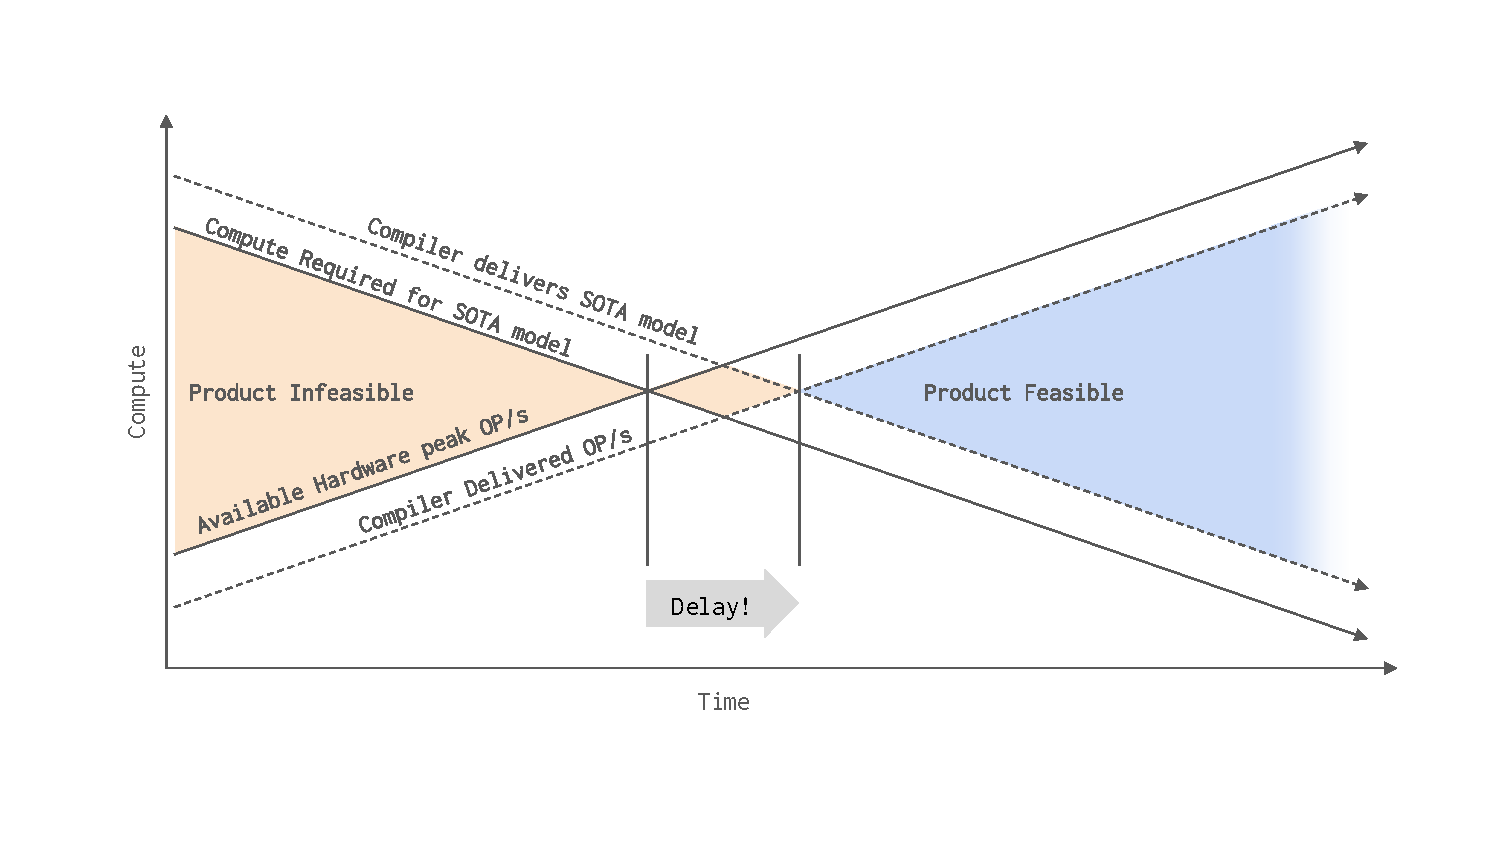
\includegraphics[width=\textwidth]{images/background/compilers_lagging.pdf}
    \caption{Compilers are lagging behind the development of both machine learning hardware and workloads. Figure created by Anton Lydike based on a slide from Sean Silva's talk at the March 2025 Cambridge Compiler Social.}
    \label{fig:compilers-lagging}
\end{figure}

% Hook
Early compilers such as Grace Hopper's A0 and the ALGOL compiler were standalone programs, specific to individual languages \cite{knuthEarlyDevelopmentProgramming1980}.
% Argument
Researchers then generalised these standalone programs into shared infrastructure, for example with the SUIF project \cite{wilsonSUIFInfrastructureResearch1994}.
The \ac{gcc} project adopted these ideas, providing a popular and open-source shared infrastructure for the compilers of several languages, including C, C++, and FORTRAN. However, its monolithic and tightly-coupled design limited the reusability of its components \cite{stallmanUsingGnuCompiler2009}, presenting a research gap in the field.
% Link
% The release of LLVM, a modular, library-based compiler framework, rejected these limitations.

\section{The LLVM project}
\label{sec:llvm}

% Hook
In 2004, Lattner and Adve published ``LLVM: A Compilation Framework for
Lifelong Program Analysis and Transformation'' \cite{lattnerLLVMCompilationFramework2004}, productising a collection of good ideas in compiler design.
% Argument
One of LLVM's key contributions was a human-readable textual \ac{ir}, contrasting the binary \acp{ir} of \texttt{gcc} at the time. This \ac{ir} has a language- and target-independent \acs{risc}-like instruction set in \ac{ssa} form \cite{cytronEfficientlyComputingStatic1991}, making LLVM re-usable across different frontends and backends, while benefitting from shared infrastructure. Modular transformation passes can be defined to modify this \ac{ir}. These passes can be composed to implement sophisticated optimisation pipelines, as each pass operates on the same \ac{ir} structures.
These desirable properties lead to LLVM's widespread adoption, but the demands of modern workloads present a number of challenges for LLVM.
% Link
For example, LLVM's low-level \ac{ir} is not well suited to abstract over the high-level operation rewrites required to optimise machine learning workloads. In addition to this key infrastructure such as parsing and printing must be implemented by hand, slowing development velocity.

\section{Multi-level intermediate representation (MLIR)}
\label{sec:mlir}

% Hook
\acf{mlir} addresses these modern challenges, providing ``compiler infrastructure for the end of Moore's law'' \cite{lattnerMLIRScalingCompiler2021a}.
% Argument
Its key contribution is allowing users to easily define multiple levels of abstraction supporting heterogeneous recursively nested structures, referred to as dialects. This contrasts the fixed low-level abstractions and homogeneous flat structures of LLVM \ac{ir}, which is less dynamic as a result of having a shape known at runtime. As a result of this, \ac{mlir} allows different problem domains to define their own operations and transformation passes while sharing common infrastructure. This facilitates efficiently expressing optimisations at the most appropriate abstraction level, which can be each by applied by lowering from high-level domain-specific representations to low-level hardware-specific ones. Lowering extensively leverages pattern rewriting, a declarative way to express transformations as patterns which match \ac{ir} constructs and replace them with lowered versions.
The provision of common infrastructure including documentation generation, parsing and printing logic, and location tracking further reduces the engineering effort required to develop complex optimisations and support custom hardware targets.
\ac{mlir} is implemented in C++, providing desirable performance characteristics, but having long build times and a verbose syntax.
% Link

% Hook
These issues are partially mitigated by \ac{irdl}, ``a domain-specific language to define \acp{ir}'' \cite{fehrIRDLIRDefinition2022a}, implemented as a \ac{ssa}-based dialect of \ac{mlir} itself.
% Argument
\ac{irdl} provides a declarative system for defining dialects, operations, and types which can be dynamically loaded at runtime, avoiding the need for verbose C++ implementations which require recompilation.
% Link

\section{xDSL}
\label{sec:xdsl}

% Hook
xDSL is a Python-native compiler framework, originally written as a re-implementation of \ac{mlir}'s data structures and associated logic.
% Argument
As a result of its similar data structures and shared textual \ac{ir}, xDSL can be used as a side-kick compiler for \ac{mlir}, facilitating modular replacement of individual components of its pipeline. This is achieved with a DSL implementation in Python of \ac{irdl}.
In contrast to \ac{mlir}, xDSL prioritises developer productivity through Python's easy-to-use syntax and fast build times, along with first-class support for user-extensibility which allows adding new operations at runtime. xDSL's implementation in Python incurs a performance cost over C++, as a consequence of the overhead of its virtual machine, and lack of support for ahead-of-time optimisations.
% Link
This trade-off has benefits for modern compiler developers, where improvements to developer productivity are critical to minimise delay for state-of-the-art workloads (\autoref{fig:compilers-lagging}). In addition to this, this thesis argues that the loss of ahead-of-time optimisations is less impactful for highly dynamic workloads such as compiler infrastructures.


\section{Dynamic languages and workloads}
\label{sec:static-dynamic-languages}

%% Define dynamism and dynamic/static languages
% Hook
Programming language design is a game of trade-offs, with a wide variety of design choices incurring differing benefits and costs.
% Argument
One such choice is the degree of dynamism, defined by Williams et al. as ``allowing properties of programs to be defined at run-time'' \cite{williamsDynamicInterpretationDynamic2010}. As such, static languages fix properties ahead of time, whereas dynamic languages offer more flexibility at runtime.
The literature of programming language design discusses these trade-offs for features including dynamic dispatch and runtime meta-programming (\autoref{sec:impact-dynamism-related-work}).
% Link

%% Dynamism of workloads
% Hook
In addition to considering support for dynamism as a property of a programming language, it can be helpful to classify a workload as dynamic or static.
% Argument
For example, \ac{gemm} operations which underpin modern machine learning systems rely on streaming data in a statically known order. This is well-suited to ahead-of-time compilation, as it is amenable to optimisation passes requiring no runtime information, such as code motion or vectorisation \cite{emerybergerPythonPerformanceMatters2022}.
In contrast, pattern rewriting in user-extensible compiler frameworks relies on pointer chasing data structures with a high degree of dynamism. The \ac{ssa} representation of the code being rewritten is structured as a doubly linked list, with the applications of the rewriting semantics to this list known only dynamically at runtime.
This dynamic, pointer-chasing workload is inherently memory bound, having irregular access patterns not amenable to traditional cache hierarchies \cite{wangEvaluatingSynchronizationOverhead2025}. Furthermore, it precludes many optimisations leveraged by ahead-of-time statically compiled languages such as C++ to accelerate their performance for other workloads.
% Link



\section{CPython internals}
\label{sec:python-internals}

%% Python reference implementation, interpreter loop, bytecode, dynamism
% Hook
Python is a high-level, dynamically typed-checked programming language, known for its readable syntax and extensive library support \cite{guidovanrossumPythonCpython2025}.
% Argument
The language has many implementations, from its reference implementation CPython to alternatives such as PyPy's \ac{jit} compiler \cite{thepypyteamPypyPypy2025}.
CPython operates by compiling Python source code into a stack-based bytecode. This bytecode is executed by a virtual machine in an interpreter loop, fetching and evaluating the compiled sequence of instructions one at a time. This approach limits performance compared with static ahead-of-time compiled languages such as C++ by the overhead of the virtual machine and having fewer opportunities for ahead-of-time optimisation. However, it also provides great flexibility, supporting Python's dynamic type system and runtime meta-programming capabilities.
% Link
The Faster CPython project is an ongoing effort to improve the performance of Python by applying techniques such as adaptive optimisation and \ac{jit} compilation.
When improving the performance of a language implementation, it is critical to have a suite of programs to measure progress. In Python, this is provided by PyPerformance, ``an authoritative source of benchmarks for all Python implementations'' \cite{collinwinterPythonPyperformance2025}.



\section{JIT compilation}
\label{sec:jit-compilation}

% Hook
In their paper ``A Brief History of Just-In-Time'', Aycock defines \acf{jit} compilation as ``translation that occurs after a program begins execution'' \cite{aycockBriefHistoryJustintime2003}.
% Argument
He argues that \ac{jit} compilation approaches aim to accrue the benefits of both ahead-of-time compilation and interpretation, combining the performance traditionally associated with compilation with the portability and access to runtime information of interpretation.
% Link

\subsection{JIT compilation to machine code}
\label{ssec:jit-compilation-machine-code}

% Hook
While \acf{jit} compilation can refer to any program translation occurring at runtime, it often refers specifically to the dynamic generation of machine code just before execution.
% Argument
Compilation during runtime exposes information from actual program behaviour which is not available to traditional ahead-of-time compilers.
% Link
This allows \ac{jit} compilers to effectively optimise the generated machine code, and unblocks the optimisation of dynamic runtimes for which there is insufficient information to optimise ahead-of-time.

%% Motivation
% Hook
A major bottleneck for traditional \ac{jit} compilation is the speed of compiler optimisation passes, which can lead to delays during program execution.
% Argument
In their paper ``Copy-and-Patch Compilation'', Xu and Kjolstad present a novel approach to avoid this runtime cost \cite{xuCopyandpatchCompilationFast2021a}, while still generating high quality machine code.
Instead of compiling code from scratch at runtime, a library of machine code stencils for common operations is constructed ahead of time, with holes left for runtime-specific information such as memory addresses. During program execution, the \ac{jit} then ``patches'' these holes to generate executable machine code without incurring the runtime cost of traditional optimising compilers such as LLVM.
% Link
%% TODO: Could talk about Deegen and luajit remake?


\subsection{Adaptive optimisation}
\label{ssec:adaptive-optimisation}

%% General case of using runtime information to change behaviour
% Hook
In addition to generating machine code on-the-fly, runtime information can be used to adapt program execution to the current workload.
% Argument
A significant overhead in the performance of dynamically typed languages is checking types at runtime, which is required to select the matching operation implementation for the type.
Whilst this type information cannot be known ahead of time in dynamically typed languages, information collected at runtime can be used to optimised the type-checking process. This adaptive optimisation approach relies on the assumption that if a variable has had a fixed type for a sufficient span of time previously, it is likely that it will have the same type in future. For example, whilst a variable being used as an integer counter in a loop can take any value, if its type in the earlier iterations has always been an integer, it is likely to remain an integer throughout later iterations.
% Link
In an interpreted language, this assumption can be leveraged to replace general instructions with faster, specialised variants. A concrete implementation of this is Python's specialising adaptive interpreter, discussed in \autoref{sec:specialising-adaptive-interpreter}.
